\documentclass[submit]{harvardml}


\course{CS181-S24}
\assignment{Assignment \#1}
\duedate{11:59pm ET, February 10, 2024} 

\usepackage[OT1]{fontenc}
\usepackage[colorlinks,citecolor=blue,urlcolor=blue]{hyperref}
\usepackage[pdftex]{graphicx}
\usepackage{graphicx}
\usepackage{caption}
\usepackage{fullpage}
\usepackage{enumitem}
\usepackage{soul}
\usepackage{amsmath}
\usepackage{amssymb}
\usepackage{color}
\usepackage{todonotes}
\usepackage{listings}
\usepackage{common}
\usepackage{framed}
\usepackage{float}
\usepackage{ifthen}

\usepackage[mmddyyyy,hhmmss]{datetime}

% Solution environment
\newenvironment{solution}
  {\color{blue}\section*{Solution}}
{}

\definecolor{verbgray}{gray}{0.9}

\lstnewenvironment{csv}{
  \lstset{backgroundcolor=\color{verbgray},
  frame=single,
  framerule=0pt,
  basicstyle=\ttfamily,
  columns=fullflexible}}{}

 \DeclareMathOperator*{\limover}{\overline{lim}}


\begin{document}
\begin{center}
{\Large Homework 1: Regression}\\
\end{center}

\subsection*{Introduction}
This homework is on different three different forms of regression:
kernelized regression, nearest neighbors regression, and linear
regression.  We will discuss implementation and examine their
tradeoffs by implementing them on the same dataset, which consists of
temperature over the past 800,000 years taken from ice core samples.

The folder \verb|data| contains the data you will use for this
problem. There are two files:
\begin{itemize}
    \item \verb|earth_temperature_sampled_train.csv| 
    \item \verb|earth_temperature_sampled_test.csv|
\end{itemize} 

Each has two columns.  The first column is the age of the ice core
sample.  The second column is the approximate difference in a year's temperature (K) 
from the average temperature of the 1,000 years preceding it. The temperatures were retrieved from ice cores in
Antarctica (Jouzel et al. 2007)\footnote{Retrieved from
\url{https://www.ncei.noaa.gov/pub/data/paleo/icecore/antarctica/epica_domec/edc3deuttemp2007.txt}

Jouzel, J., Masson-Delmotte, V., Cattani, O., Dreyfus, G., Falourd, 
S., Hoffmann, G., … Wolff, E. W. (2007). Orbital and Millennial 
Antarctic Climate Variability over the Past 800,000 Years. 
\emph{Science, 317}(5839), 793–796. doi:10.1126/science.1141038}.
 
The following is a snippet of the data file:
 
\begin{csv}
# Age, Temperature
399946,0.51
409980,1.57
\end{csv}

\noindent And this is a visualization of the full dataset: 
\begin{center}
  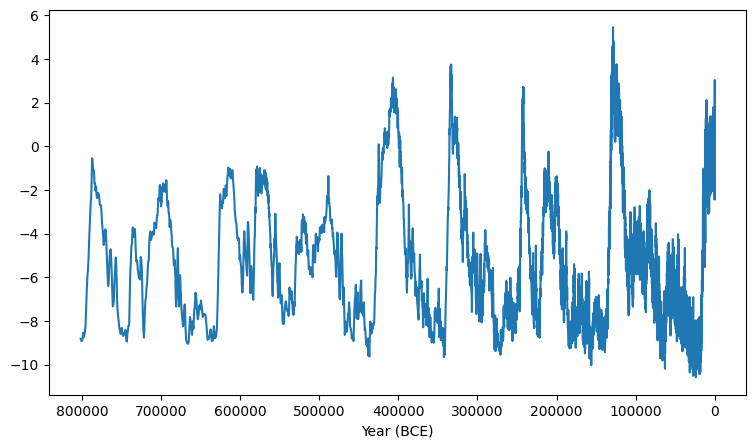
\includegraphics[width=.8\textwidth]{images/sample_graph}
    \end{center}
  \noindent 


\textbf{Due to the large magnitude of the years, we will work in terms
  of thousands of years BCE in Problems 1-3.} This is taken care of
for you in the provided notebook.






\subsection*{Resources and Submission Instructions}
If you find that you are having trouble with the first couple
problems, we recommend going over the fundamentals of linear algebra
and matrix calculus (see links on website).  The relevant parts of the
\href{https://github.com/harvard-ml-courses/cs181-textbook/blob/master/Textbook.pdf}{cs181-textbook
  notes are Sections 2.1 - 2.7}.  We strongly recommend reading the
textbook before beginning the homework.

We also encourage you to first read the
\href{http://users.isr.ist.utl.pt/~wurmd/Livros/school/Bishop\%20-\%20Pattern\%20Recognition\%20And\%20Machine\%20Learning\%20-\%20Springer\%20\%202006.pdf}{Bishop
  textbook}, particularly: Section 2.3 (Properties of Gaussian
Distributions), Section 3.1 (Linear Basis Regression), and Section 3.3
(Bayesian Linear Regression). (Note that our notation is slightly
different but the underlying mathematics remains the same!).

\textbf{Please type your solutions after the corresponding problems
  using this \LaTeX\ template, and start each problem on a new page.}
You may find the following introductory resources on \LaTeX\ useful:
\href{http://www.mjdenny.com/workshops/LaTeX_Intro.pdf}{\LaTeX\ Basics}
and
\href{https://www.overleaf.com/learn/latex/Free_online_introduction_to_LaTeX_(part_1)}{\LaTeX\ tutorial
  with exercises in Overleaf}

Homeworks will be submitted through Gradescope. You will be added to
the course Gradescope once you join the course Canvas page. If you
haven't received an invitation, contact the course staff through Ed.

\textbf{Please submit the writeup PDF to the Gradescope assignment
  `HW1'.} Remember to assign pages for each question.

\textbf{Please submit your \LaTeX file and code files to the
  Gradescope assignment `HW1 - Supplemental'.} Your files should be
named in the same way as we provide them in the repository,
e.g. \texttt{hw1.pdf}, etc.


%%%%%%%%%%%%%%%%%%%%%%%%%%%%%%%%%%%%%%%%%%%%%
% Problem 1
%%%%%%%%%%%%%%%%%%%%%%%%%%%%%%%%%%%%%%%%%%%%%
\newpage

\begin{problem}[Setting up the Regression, 10pts]
As noted in the introduction, your goal is to predict temperature
variation given the year.  Before we start deriving and coding up our
regressions, we will interrogate the set-up of our problem.  

\begin{enumerate}
  \item These data were derived from ice core samples in Antarctica.
    Take a brief look at the
    \href{https://www.ncei.noaa.gov/pub/data/paleo/icecore/antarctica/epica_domec/edc3deuttemp2007.txt}{original
      data file}.  Briefly discuss how the data were processed: what kinds of
    decisions and corrections had to be made?  We know that different
    places on earth have different temperatures: what does the
    temperature in the temperature column correspond to?
        
  \item Even before doing any formal regressions, we see that there is
    some periodicity in the data: there are years that are warmer, and
    years that are cooler.  Suppose you are a government official
    advising on how much to worry about climate change.  Would it be
    reasonable to use this pattern as evidence that the earth will
    cool down again?  Why or why not, or to what extent?


  \item In the problems below, we will focus on interpolating
    temperatures for years not provided in the training set.  What
    kind of application would such a regression be useful for? 

\end{enumerate}
  
\end{problem}

% qwer
\newpage
\begin{solution}
	\textbf{1.} The data in this dataset was processed by looking at the concentration 
  of Deuterium in ice cores and using that concentration along with the chronological
  age of the ice to estimate the temperatures at the time that the ice was formed. 
  In this case, since they were taking samples across various points, the scientists 
  decided to make corrections according to the elevation of the sample and sea-water interference.
  The temperature in the temperature column is the difference between a year's temperature as compared 
  with the previous 1000 years before it. Essentially, this makes temperature a measure of how much 
  temperature has increased relative to the average.\\\\

  \textbf{2.} It would not be advisable to preach the ability of using this graph to justify 
  earth cooling down again because even the most recent entries in this list are over 2000 years old, 
  and the pattern of warming and cooling could have changed in that time. It could be helpful instead to 
  look at a graph that plots the same thing as the given graph but for the last two centuries so that we can more correctly 
  see if something is artificially ruining the map or if the modern extension still follows the same trends we 
  would expect it to. It is reasonable to say that we expect that the earth will cool again, but until we can 
  see the graph for the last two thousand years, it seems dangerous to say that it will unequivocally. \\\\

  \textbf{3.} That is helpful for the situation I was describing above, where we want to see what a predicted periodic function looks like
  and extending it to the present day so we can compare what is actually occuring with what
  we expected to occur and assign some sort of causality to the problem. 
\end{solution}
% rewq
\newpage

%%%%%%%%%%%%%%%%%%%%%%%%%%%%%%%%%%%%%%%%%%%%%
% Problem 2
%%%%%%%%%%%%%%%%%%%%%%%%%%%%%%%%%%%%%%%%%%%%%

\begin{problem}[Optimizing a Kernel, 30pts]
Kernel-based regression techniques are similar to nearest-neighbor
regressors: rather than fit a parametric model, they predict values
for new data points by interpolating values from existing points in
the training set.  In this problem, we will consider a kernel-based
regressor of the form:
\begin{equation*}
  f_\tau(x^*) = \cfrac{\sum_{n} K_\tau(x_n,x^*) y_n}{\sum_n K_\tau(x_n, x^*)} 
\end{equation*}
where $\mathcal{D}_\texttt{train} = \{(x_n,y_n)\}_{n = 1} ^N$ are the
training data points, and $x^*$ is the point for which you want to
make the prediction.  The kernel $K_\tau(x,x')$ is a function that
defines the similarity between two inputs $x$ and $x'$. A popular
choice of kernel is a function that decays as the distance between the
two points increases, such as
\begin{equation*}
  K_\tau(x,x') = \exp\left\{-\frac{(x-x')^2}{\tau}\right\}
\end{equation*}
where $\tau$ represents the square of the lengthscale (a scalar value that 
dictates how quickly the kernel decays).  In this
problem, we will consider optimizing what that (squared) lengthscale
should be. 

\noindent\emph{Make sure to include all required plots in your PDF.}

\begin{enumerate}
  
\item Let's first take a look at the behavior of the fitted model for different values of $\tau$. Implement the \texttt{kernel\_regressor} function in the notebook, and plot your model for years in the range $800,000$ BC to $400,000$ BC at $1000$ year intervals for the following three values of $\tau$: $1, 50, 2500$. Since we're working in terms of thousands of years, this means you should plot $(x, f_\tau(x))$ for $x = 400, 401, \dots, 800$. \textbf{The plotting has been set up} for you in the notebook already.

Include your plot in your solution PDF.

\textbf{In no more than 5 sentences}, describe how the fits change with $\tau$.

\item Now, we will evaluate the quality of each model \emph{quantitatively} by computing the error on some test set $\mathcal{D}_\texttt{test} = \{(x'_m, y'_m)\}_{m = 1} ^M$.  Write down the expression for MSE of $f_\tau$ over the test set as a function of the training set and test set. Your answer may include $\{(x'_m, y'_m)\}_{m = 1} ^M$, $\{(x_n, y_n)\}_{n = 1} ^N$, and $K_\tau$, but not $f_\tau$.

\item Suppose we used the training set as our test set, that is, we evaluated the expression above with $\mathcal{D}_\texttt{test} = \mathcal{D}_\texttt{train}$, and chose the value of $\tau$ which gave the smallest loss.  What value of $\tau$ would be picked?  Why is setting $\mathcal{D}_\texttt{test} = \mathcal{D}_\texttt{train}$ a bad idea?
   
\emph{Hint: consider what value of $\tau$ would be optimal, for $\tau$ ranging in $(0, \infty)$. We can consider $f_\tau(x^*)$ as a weighted average of the training responses, where the weights are proportional to the distance to $x^*$, and the distance is computed via the kernel. What happens to $K_\tau(x, x')$ as $\tau$ becomes very small, when $x = x'$? What about when $x \neq x'$?}

\item Let us compute the MSE on the provided test set (that is, not the training set). Write Python code to compute the MSE with respect to the same lengthscales as in Part 1. Which model yields the lowest test set MSE? 

\item Describe the time and space complexity of kernelized regression with respect to the size of the training set $N$.  How, if at all, does the size of the model---everything that needs to be stored to make predictions---change with the size of the training set $N$?  How, if at all, do the number of computations required to make a prediction for some input $x^*$ change with the size of the training set $N$?

\end{enumerate}

\end{problem}


% qwer
\newpage
\begin{figure}
  \centering
  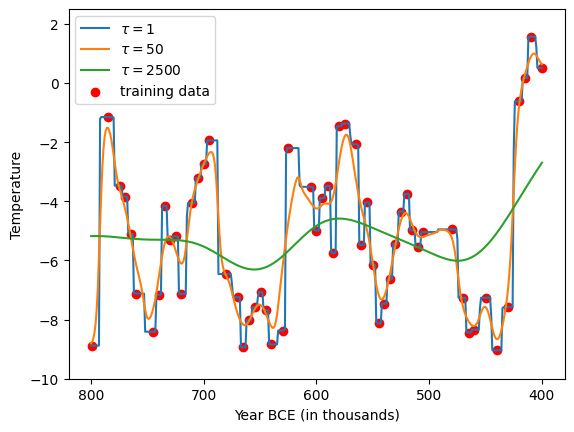
\includegraphics[width=0.4\textwidth]{tau_plot.png}
\end{figure}

\begin{solution}
	\textbf{1.} The plot for this Kernel Regression with respect to the values 
  $\tau = 1, 50, 2500$ is shown above. As you can see in the graph, as Tau increases, the squared error also increases. When $\tau = 1$, the line goes through
  every data point, creating a squared error of 0. Then when $\tau$ is increased to 50, the line is still very accurate and goes through most points, 
  but has some value for the squared error. Most notably, when $\tau = 50$ the line rarely passes through points which are local extrema. This pattern continues when 
  we once again increase tau to be equal to 2500, where we see that the line has a much greater squared error and does not go through many points specifically. \\\\

  \textbf{2.} To begin this problem, it is important to consider it in terms of $f_\tau(x)$. To find the MSE of the data set, we need to do $\frac{1}{M} \sum_{m=1}^{M}(y'_m - f_\tau(x'_m))^2$. 
  We can then substitute for the equation of $f_\tau(x)$ that we used in Part 1 to get that 
  MSE = $\frac{1}{M} \sum_{m=1}^{M}[y'_m - \frac{\sum_{n=1}^{N}(K_\tau(x_n,x'_m)y_n)}{\sum_{n=1}^{N}(K_\tau(x_n, x'_m))}]^2$. And this is in terms of $K_\tau, D_{test},$ and $D_{train}$ but not 
  $f_\tau$. \\\\

  \textbf{3.} If we use the training set as our test set, the value of $\tau$ that would give the 
  smallest loss would be a value such that $\tau \approx 0$. This is because as the value of $\tau$ gets smaller,
  the denominator of the exponential in $K_T$ gets smaller and produces values closer and closer to 1, meaning that two points 
  such that $x = x'$ are assigned a very high similarity. On the other hand, if $x \neq x'$, then $K_\tau$ assigns a very low
  similarity between the two points. What this does is that it causes a lot of overfitting on the curve as any slight difference between 
  points gets a high value for the MSE and so the line passes through every point, being useless for generalizations. \\\\

  \textbf{4.} When I computed the values of MSE for the various values of $\tau$, I got the results: 
  [tau = 1: loss = 1.9472621565209178], [tau = 50: loss = 1.8582899169613447], [tau = 2500: loss = 8.333886806980791]. 
  This means that the model that yields the least MSE is the value $\tau = 50$. \\\\

  \textbf{5.} The time and space complexity with respect to the size of N for kernelized regression is that 
  as the data set grows, the time it takes to calculate the regression also increases linearly. This is because the equation for 
  kernelized regression involves multiple sums that sum over all of the data points individually. Each sum operates on O(N), but when also 
  the kernelized regression operates with pairwise sum as well which operates on the order of $O(N^2)$. The amount of computations is similarly related, 
  being tied with the amount of sums that have to be taken as directly influenced by the size of N.
\end{solution}
\newpage
% rewq

%%%%%%%%%%%%%%%%%%%%%%%%%%%%%%%%%%%%%%%%%%%%%
% Problem 3
%%%%%%%%%%%%%%%%%%%%%%%%%%%%%%%%%%%%%%%%%%%%%

\newpage
\begin{problem}[Kernels and kNN, 20pts]

Now, let us compare the kernel-based approach to an approach based on
nearest-neighbors.  Recall that kNN uses a predictor of the form
  \begin{equation*}
    f(x^*) = \frac{1}{k} \sum_n y_n \mathbb{I}(x_n \texttt{ is one of k-closest to } x^*)
  \end{equation*}

\noindent where $\mathbb{I}$ is an indicator variable. For this problem, you will use the \textbf{same dataset as in Problem 1}.


%\textbf{For this problem, you may also use the second half of the notebook at {\color{red} update name} \texttt{T1\_P1-2.ipynb}.} 

\textbf{Note that our set of test cases is not comprehensive: just because you pass does not mean your solution is correct! We strongly encourage you to write your own test cases and read more about ours in the comments of the Python script.}

\vspace{0.5cm}
\noindent\emph{Make sure to include all required plots in your PDF.}


\begin{enumerate}

\item The kNN implementation \textbf{has been provided for you} in the notebook. Run the cells to plot the results for $k=\{1, 3, N-1\}$, where $N$ is the size of the dataset.

  Describe what you see: what is the behavior of the functions in
  these three plots?  How does it compare to the behavior of the
  functions in the three plots from Problem 1? In particular, are
  there situations in which kNN and kernel-based regression
  interpolate similarly?

\item Compute the MSE on the test set for each value of $k$.  Which solution has the lowest MSE?  

\item As in Problem 1, describe the space and time complexity of kNN.  How does what is stored to compute predictions change with the size of the training set $N$?  How does the computation needed to compute the prediction for a new input depend on the size of the training set $N$? (For the latter, justify based off of your implementation.)

\end{enumerate}

\end{problem}


% qwer
\newpage
\begin{solution}
	\textbf{1. } The behavior of the functions for $k = 1, 3, N - 1$ is very similar 
  to the observed behaviors of kernelized regression with values $\tau = 1, 50, 2500$. 
  With $k = 1$, the regression line has almost no error and goes through all of the training data exactly, 
  resulting in a very jagged and unnatural line. With $k=3$, the line is still 
  passing through most points in the training data, but it has more deviation from the points. 
  This is especially prevalent in areas where there are multiple points congregated around a similar area, 
  in which case the line at $k = 3$ gravitates towards those clumps, mainly ignoring extra. Then with the case
  of $k = N - 1$, the resulting line is not very accurate to the data point and is instead
  squarely in the middle of the distribution. \\\\

  \textbf{2. } When I computed the MSE on the test set for each value of k, I got the following: 
  [k = 1: MSE loss = 1.7406000000000004].
  [k = 3: MSE loss = 3.890766222222223],
  [k = 55: MSE loss = 9.66397324033058],
  [k = 56: MSE loss = 9.528571442602042]. Based on these numbers, the solution with the lowest MSE is $k = 1$, 
  which makes sense because that is the most direct method of relating it to the point directly adjacent to it which leads
  to almost no error. 

  \textbf{3. } Since kNN is only interested in individual points and their relationships with neighbors, the 
  complexity of both the time and space of KNN regression is on the order O(N). This means that as the dataset increases to a value N, 
  the time and complexity will increase linearly with the increase in data points. 
\end{solution}
\newpage
% rewq


%%%%%%%%%%%%%%%%%%%%%%%%%%%%%%%%%%%%%%%%%%%%%
% Problem 4
%%%%%%%%%%%%%%%%%%%%%%%%%%%%%%%%%%%%%%%%%%%%%

\newpage
\begin{problem}[Modeling Climate Change 800,000 Years Ago, 30pts]

Our last regression will be linear regression.  We currently only have
a one dimensional input, the year.  To create a more expressive linear
model, we will introduce basis functions.
\vspace{1em}
\noindent\emph{Make sure to include all required plots in your PDF.}

\begin{enumerate}
\item 
We will first implement the four basis regressions below. (The first basis has been implemented for you in the notebook as an example.) Note that we introduce an addition transform $f$ (already into the provided notebook) to address concerns about numerical instabilities.
\begin{enumerate}
  \item $\phi_j(x)= f(x)^j$ for $j=1,\ldots, 9$. $f(x) = \frac{x}{1.81 \cdot 10^{2}}.$
  \item $\phi_j(x) = \exp\left\{-\cfrac{(f(x)-\mu_j)^2}{5}\right\}$ for $\mu_j=\frac{j + 7}{8}$ with $j=1,\ldots, 9$. $f(x) = \frac{x}{4.00 \cdot 10^{2}}.$
  \item $\phi_j(x) =  \cos(f(x) / j)$ for $j=1, \ldots, 9$. $f(x) = \frac{x}{1.81}$.
  \item $\phi_j(x) = \cos(f(x) / j)$ for $j=1, \ldots, 49$. $f(x) = \frac{x}{1.81 \cdot 10^{-1}}$. \footnote{For the trigonometric bases (c) and (d), the periodic nature of
cosine requires us to transform the data such that the 
lengthscale is within the periods of each element of our basis.}
\end{enumerate}

{\footnotesize * Note: Please make sure to add a bias term for
all your basis functions above in your implementation of the 
\verb|make_basis|.}

Let 
$$ \mathbf{\phi}(\mathbf{X}) = 
\begin{bmatrix} 
\mathbf{\phi}(x_1) \\
\mathbf{\phi}(x_2) \\
\vdots \\
\mathbf{\phi}(x_N) \\
\end{bmatrix} \in \mathbb{R}^{N\times D}.$$
You will complete the \verb|make_basis| function which must return
$\phi(\mathbf{X})$ for each part 
(a) - (d). You do NOT need to submit this
code in your \LaTeX writeup.

For each basis create a plot of your code graphing the least squares
regression line trained on your training data against a scatter plot
of the training data. Boilerplate plotting code is provided in the
notebook.
\textbf{All you need to include 
in your writeup for this part are these four plots.}
\vspace{1em}
\end{enumerate}
\end{problem}


\newpage
\begin{framed}
\noindent\textbf{Problem 4} (cont.)\\
\begin{enumerate}
\setcounter{enumi}{1}
\item 
Now we have trained each of our basis regressions.  For each basis
regression, compute the MSE on the test set.  Discuss: do any of the
bases seem to overfit?  Underfit?  Why?

% \item Make a claim regarding whether this basis overfits, 
% underfits, or fits well. Write 1-2 sentences explaining your 
% claim using the train and test negative log-likelihood and MSE.

% \end{itemize}

\item Briefly describe what purpose the transforms $\phi$ serve: why are they helpful?

\item As in Problems 1 and 2, describe the space and time complexity of linear regression.  How does what is stored to compute predictions change with the size of the training set $N$?  How does the computation needed to compute the prediction for a new input depend on the size of the training set $N$?  How do these complexities compare to those of the kNN and kernelized regressor?

\item Briefly compare and constrast the different regressors: kNN,
  kernelized regression, and linear regression (with bases).  Are some
  regressions clearly worse than others?  Is there one best
  regression?  How would you use the fact that you have these multiple
  regression functions?
  
\end{enumerate}
Note:
Recall that we are using a 
different set of inputs $\mathbf{X}$ for each basis (a)-(d). 
Although it may seem as though this prevents us from being able 
to directly compare the MSE since we are using different data, 
each transformation can be considered as being a part of our model. 
Contrast this with transformations (such as standardization) that cause the variance of the target $\mathbf{y}$ to be different; in these cases the
MSE can no longer be directly compared.

\end{framed}
\newpage
% qwer
\begin{figure}
  \centering
  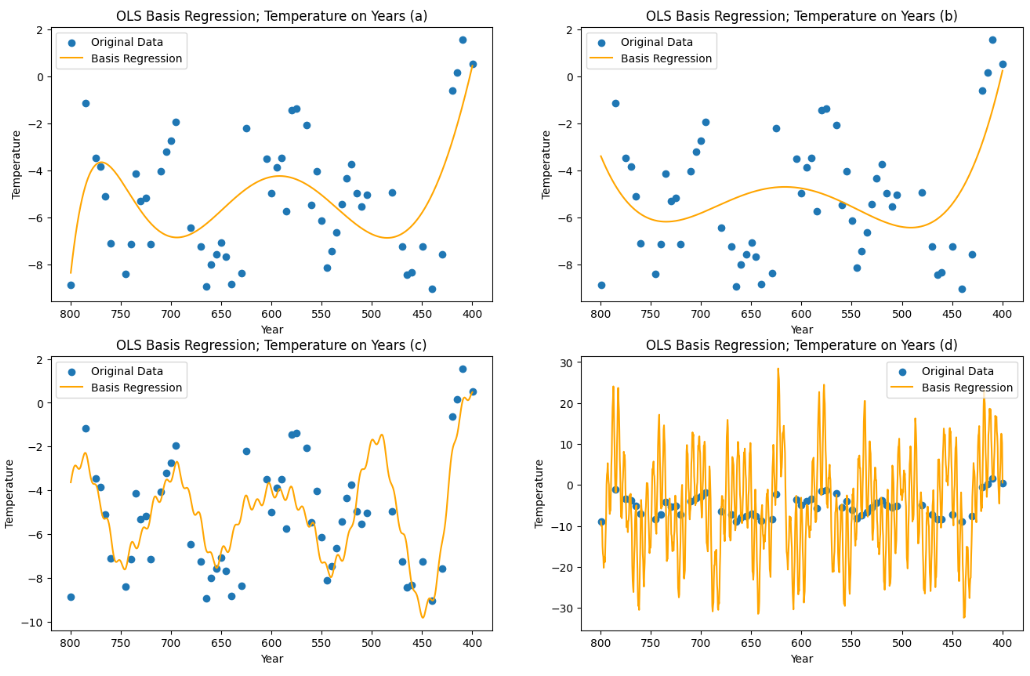
\includegraphics[width=0.4\textwidth]{Linear_bases.png}
\end{figure}

\begin{solution}
  \textbf{1.} Image above.

  \textbf{2.} Part (a): Train MSE: 4.82; Test MSE: 5.72 \\ Part (b): Train MSE: 5.53; Test MSE: 6.47 \\
  Part (c): Train MSE: 2.88; Test MSE: 4.55 \\ Part (d): Train MSE: 0.64; Test MSE: 0.00 \\
  From these values, it is evident that Test d has the least MSE, which is surprising to me because that graph seems to be entirely overfitted, 
  being so complex that it has to even stretch out the range of the graph. It seems like graph B underfits the data because it has the most standard 
  error. Part c is a good mix of the two, with the data being well fit but having a small mse.

  \textbf{3.} The transforms $\phi$ serve as a basis for the linear regression so that the resulting regression line doesn't need to be linear
  but instead can be linear with respect to the basis, resulting in more advanced regression lines. What the phi is determines the kind of 
  graph that ultimately results when you do the regression and so can impact mean squared error. 

  \textbf{4.} With a training size of N, linear regression increases on the order O(N) because each new data point only adds one more calculation,
  rather than the more complex results with KNN or Kernel. The same is true for both the space and the time. 

  \textbf{5.} kNN, Kernelized, and Linear regression are all helpful ways to fit datapoints, but each comes with their own drawbacks. Performance wise, 
  when you compare the best test that is not overfit across all three methods of regression, we find that for kernelized regression, the best value is 1.84, 
  being a very small value for MSE, kNN offered an optimal MSE of 3.89, which is worse, and linear provided a minimum mse of 4.55, which is the worst. 
  This also agrees with our discussions in class because kNN is just a simpler version of kernelized, and both are more advanced than the linear methods. 
  As the level of complexity increases, the mean squared error decreases, which aligns with what we've went over in class. 
 
\end{solution}

\newpage
% rewq

%%%%%%%%%%%%%%%%%%%%%%%%%%%%%%%%%%%%%%%%%%%%%
% Problem 5
%%%%%%%%%%%%%%%%%%%%%%%%%%%%%%%%%%%%%%%%%%%%%
\newpage
\begin{problem}[Deriving Linear Regression, 10pts]

  In the previous problems, you focused on implementing regressions
  and exploring their fits on data. Now we will turn to some more
  analytic work.  Specifically, the solution for the least squares
  linear regressions ``looks'' kind of like a ratio of covariance and
  variance terms.  In this problem, we will make that connection more
  explicit. \\

  \noindent Let us assume that our data are tuples of scalars $(x,y)$ that are
  described by some joint distribution $p(x,y)$.  For clarification, the joint distribution $p(x,y)$ is just another way of saying the ``joint PDF'' $f(x,y)$, which may be more familiar to those who have taken Stat 110, or equivalent. \\
  
  \noindent We will consider the process of fitting these data from this distribution with the best linear model
  possible, that is a linear model of the form $\hat{y} = wx$ that
  minimizes the expected squared loss $E_{x,y}[ ( y - \hat{y} )^2
  ]$.\\

\noindent \emph{Notes:} The notation $E_{x, y}$ indicates an
expectation taken over the joint distribution $p(x,y)$.  Since $x$ and
$y$ are scalars, $w$ is also a scalar.
  
  \begin{enumerate}

  \item Derive an expression for the optimal $w$, that is, the $w$
    that minimizes the expected squared loss above.  You should leave
    your answer in terms of moments of the distribution, e.g. terms
    like $E_x[x]$, $E_x[x^2]$, $E_y[y]$, $E_y[y^2]$, $E_{x,y}[xy]$
    etc.

\item Provide unbiased and consistent formulas to estimate $E_{x, y}[yx]$
 and $E_x[x^2]$ given observed data $\{(x_n,y_n)\}_{n=1}^N$.

\item In general, moment terms like $E_{x, y}[yx]$, $E_{x, y}[x^2]$,
  $E_{x, y}[yx^3]$, $E_{x, y}[\frac{x}{y}]$, etc. can easily be
  estimated from the data (like you did above).  If you substitute in
  these empirical moments, how does your expression for the optimal
  $w^*$ in this problem compare with the optimal $w^*$ that we see in
  Section 2.6 of the cs181-textbook?

\item Many common probabilistic linear regression models assume that
  variables x and y are jointly Gaussian.  Did any of your above
  derivations rely on the assumption that x and y are jointly
  Gaussian?  Why or why not?
    
\end{enumerate}
  
\end{problem}

\newpage
\begin{solution}
	Your solution here.
\end{solution}

%%%%%%%%%%%%%%%%%%%%%%%%%%%%%%%%%%%%%%%%%%%%%
% Name and Calibration
%%%%%%%%%%%%%%%%%%%%%%%%%%%%%%%%%%%%%%%%%%%%%
\newpage
\subsection*{Name:} Dan Tracy

\subsection*{Collaborators and Resources}
Whom did you work with, and did you use any resources beyond cs181-textbook and your notes? \\
N/A

\end{document}